% This is "sig-alternate.tex" V2.0 May 2012
% This file should be compiled with V2.5 of "sig-alternate.cls" May 2012
%
% This example file demonstrates the use of the 'sig-alternate.cls'
% V2.5 LaTeX2e document class file. It is for those submitting
% articles to ACM Conference Proceedings WHO DO NOT WISH TO
% STRICTLY ADHERE TO THE SIGS (PUBS-BOARD-ENDORSED) STYLE.
% The 'sig-alternate.cls' file will produce a similar-looking,
% albeit, 'tighter' paper resulting in, invariably, fewer pages.
%
% ----------------------------------------------------------------------------------------------------------------
% This .tex file (and associated .cls V2.5) produces:
%       1) The Permission Statement
%       2) The Conference (location) Info information
%       3) The Copyright Line with ACM data
%       4) NO page numbers
%
% as against the acm_proc_article-sp.cls file which
% DOES NOT produce 1) thru' 3) above.
%
% Using 'sig-alternate.cls' you have control, however, from within
% the source .tex file, over both the CopyrightYear
% (defaulted to 200X) and the ACM Copyright Data
% (defaulted to X-XXXXX-XX-X/XX/XX).
% e.g.
% \CopyrightYear{2007} will cause 2007 to appear in the copyright line.
% \crdata{0-12345-67-8/90/12} will cause 0-12345-67-8/90/12 to appear in the copyright line.
%
% ---------------------------------------------------------------------------------------------------------------
% This .tex source is an example which *does* use
% the .bib file (from which the .bbl file % is produced).
% REMEMBER HOWEVER: After having produced the .bbl file,
% and prior to final submission, you *NEED* to 'insert'
% your .bbl file into your source .tex file so as to provide
% ONE 'self-contained' source file.
%
% ================= IF YOU HAVE QUESTIONS =======================
% Questions regarding the SIGS styles, SIGS policies and
% procedures, Conferences etc. should be sent to
% Adrienne Griscti (griscti@acm.org)
%
% Technical questions _only_ to
% Gerald Murray (murray@hq.acm.org)
% ===============================================================
%
% For tracking purposes - this is V2.0 - May 2012

\documentclass{sig-alternate}

\begin{document}
%
% --- Author Metadata here ---
% Allows default copyright year (20XX) to be over-ridden - IF NEED BE.
%\crdata{0-12345-67-8/90/01}  % Allows default copyright data (0-89791-88-6/97/05) to be over-ridden - IF NEED BE.
% --- End of Author Metadata ---

\title{State of the Art in Crowdsourcing
}
%
% You need the command \numberofauthors to handle the 'placement
% and alignment' of the authors beneath the title.
%
% For aesthetic reasons, we recommend 'three authors at a time'
% i.e. three 'name/affiliation blocks' be placed beneath the title.
%
% NOTE: You are NOT restricted in how many 'rows' of
% "name/affiliations" may appear. We just ask that you restrict
% the number of 'columns' to three.
%
% Because of the available 'opening page real-estate'
% we ask you to refrain from putting more than six authors
% (two rows with three columns) beneath the article title.
% More than six makes the first-page appear very cluttered indeed.
%
% Use the \alignauthor commands to handle the names
% and affiliations for an 'aesthetic maximum' of six authors.
% Add names, affiliations, addresses for
% the seventh etc. author(s) as the argument for the
% \additionalauthors command.
% These 'additional authors' will be output/set for you
% without further effort on your part as the last section in
% the body of your article BEFORE References or any Appendices.

\numberofauthors{3} %  in this sample file, there are a *total*
% of EIGHT authors. SIX appear on the 'first-page' (for formatting
% reasons) and the remaining two appear in the \additionalauthors section.
%
\author{
% You can go ahead and credit any number of authors here,
% e.g. one 'row of three' or two rows (consisting of one row of three
% and a second row of one, two or three).
%
% The command \alignauthor (no curly braces needed) should
% precede each author name, affiliation/snail-mail address and
% e-mail address. Additionally, tag each line of
% affiliation/address with \affaddr, and tag the
% e-mail address with \email.
%
% 1st. author
\alignauthor
Richard Bayerle\\
       \affaddr{Technical University of Vienna}\\
       \affaddr{Studentnr. 1025259}\\
       \email{e1025259@
       student.tuwien.ac.at}
% 2nd. author
\alignauthor
Peter Klein\\
       \affaddr{Technical University of Vienna}\\
       \affaddr{Studentnr. 8251105}\\
       \email{e8251105@
       student.tuwien.ac.at}
% 3rd. author
\alignauthor
Alexander Kumbeiz\\
       \affaddr{Technical University of Vienna}\\
       \affaddr{Studentnr. 1228689}\\
       \email{e1228689@
       student.tuwien.ac.at}
}
% There's nothing stopping you putting the seventh, eighth, etc.
% author on the opening page (as the 'third row') but we ask,
% for aesthetic reasons that you place these 'additional authors'
% in the \additional authors block, viz.
\additionalauthors{Additional authors: John Smith (The Th{\o}rv{\"a}ld Group,
email: {\texttt{jsmith@affiliation.org}}) and Julius P.~Kumquat
(The Kumquat Consortium, email: {\texttt{jpkumquat@consortium.net}}).}
\date{30 July 1999}
% Just remember to make sure that the TOTAL number of authors
% is the number that will appear on the first page PLUS the
% number that will appear in the \additionalauthors section.

\maketitle
\begin{abstract}
This paper provides an overview in the state of the art in crowd sourcing applications. A classification of crowd sourcing systems is shown according to the collaboration provided by users and the tasks performed by them. Then most important issues in building crowd sourcing systems such as recruiting and retaining users, define tasks for the users, combining results provided by users and evaluating their results are presented.
\end{abstract}

% A category with the (minimum) three required fields
\category{H.4}{Information Systems Applications}{Miscellaneous}
%A category including the fourth, optional field follows...

\terms{Internet Computing}

\keywords{ACM proceedings, \LaTeX, text tagging}

\section{Overview}
Crowd sourcing, which is utilizing a crowd of humans to solve a task that is typically easy to solve for humans but hard for machines, has to handle following 4 major tasks.
\begin{itemize}
\item Recruiting and retaining users
\item Define what the users should do
\item Combining users results
\item Evaluate the results
\end{itemize}
First step in evaluation and categorization of crowd sourcing systems is to classify them according to the type of collaboration and the task performed.
\newline\newline
\subsection{User Collaboration}
\textit{Explicit collaboration} requires users to willingly participate in creation of artifacts or solving of problems, such as writing Wikipedia articles or reviewing and voting products on Amazon
\newline\newline
\textit{Implicit collaboration} means that users are collaborating by working on other tasks such as playing games or browsing websites.
\subsection{Tasks}
\subsubsection{Explicit Systems}
\textit{Evaluation Systems} let users analyze and comment on items such as books, movies or webpages. The result can be given in textual comments, number scores or tags.
\newline\newline
\textit{Sharing Systems} lets users share items such as products, services or textual and structured knowledge. Systems that share products and services are YouTube, programmableweb.com or CPAN. Systems that share textual knowledge are QA web sites (such as Yahoo Answers) and customer support systems (such as Ask Jeeves' AnswerPoint). Systems that share structured knowledge include Swivel, Google Fusion Tables and many science web sites (such as galaxyzoo.org). Sharing systems can be central such as YouTube or working in a peer-to-peer fashion such as Orchestra.
\newline\newline
\textit{Building Artifacts} Such systems allow users to build textual knowledge bases, structured knowledge bases and software. Example of a textual knowledge base is Wikipedia where users contribute texts and web pages and edit and merge each others contributions. Structured knowledge bases include DBpedia that is based on Wikipedia info boxes, Freebase.com that builds a structured database and Google Fusion Tables that lets users contribute tabular data and collaborate on it by merging tables and commenting on them. Building a structured knowledge base requires selecting a set of data sources, extracting data from them and integrating and merging them. Users can contribute by selecting data sources, integrating structured data, resolving ambiguities and adding inferences. The most well known artifact besides Wikipedia is open source software whether users contribute by writing source code, documentation and test of the software.
\newline\newline
\textit{Task Execution Systems} let users perform collaborative tasks such as searching for missing people on images or running election campaigns to mobilize voters. A number of crowd sourcing platforms on the  web such as Amazons Mechanical Turk help distribute pieces of tasks to a crowd and collect the results.
\subsubsection{Implicit Systems}
\textit{Standalone Systems} provide a service so that users utilizing this service collaborate to solve a problem. E.g. the ESP game lets users play a game of guessing common words that describe images, those are then used to label the images. IMDB lets users import movies in a way that it motivates users to rate this movies. reCAPTCHA asks users to solve captchas to prove they are human and uses the results for handwritten digit recognition.
\newline\newline
\textit{Piggyback Systems} utilize user traces of other systems to perform a task. Many such systems have been built on top of search engines such as Google or Bing to predict epidemics or find synonyms. Other examples use traces of purchases to recommend products or use click logs to improve presentation of a web site.
\begin{figure}[h]
	\centering
	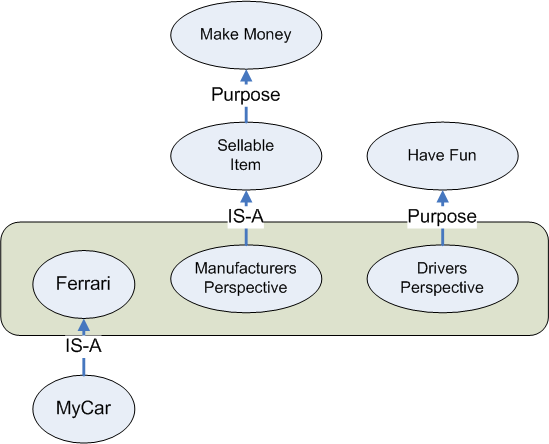
\includegraphics[width=0.4\textwidth]{perspectives}
	\caption{Logic Formulas}
      \label{fig:logic_formulas}
\end{figure}
\section{Key Issues}
\subsection{Recruiting and Retaining Users}
This is the most important crowd sourcing challenge to solve when running such a system. Following solutions can be distinguished.
\begin{itemize}
\item \textit{Requires Users} to make contributions. E.g. in an in house system management may order users to enter their contributions.
\item \textit{Pay Users} This is a very simple solution but not effective in economic sense if the services provided by the users are not very valuable. E.g. Amazons Mechanical Turk provides a way to pay users.
\item \textit{Ask for Volunteers} This is the most popular solution since it is free and easy to execute but it is hard to predict and achieve that enough contributors are found for an application.
\item \textit{Let Users "pay" for the Service} This works for implicit systems where users are only allowed to use the real service behind if they have contributed to the crowd sourcing system before.
\item \textit{Piggyback on Existing Systems} This gives a steady stream of users but only can only be applied to problems that can be solved by the existing user traces.
\end{itemize}
When the users have been acquired the next step is to encourage and retain them. Popular schemes are \textit{Instant Gratification} to give users immediate feedback on their contributions and show them the positive effects, \textit{Enjoyable Experience} e.g. to allow playing a game for a contribution,\textit{Reputation} to establish, measure and show fame and trust, this can be a very strong means to encourage users,\textit{Set up Competitions} e.g. show top rated users and provide \textit{Ownership Situations} where users feel they own part of the system.
\subsection{User Contributions}
In many crowd sourcing system contributions users can made are limited to simple tasks like reviewing, rating or tagging but in more complex systems users do much more cognitively challenging tasks, e.g providing inference rules or resolving controversial issues in building structured knowledge bases.Often users are classified in groups such as guests, regulars, editors and administrators. Low ranking users provide easy contributions such as editing a paragraph or flagging incorrect ones where as high ranking users take the hard parts. 
\newline\newline
In addition it important to quantify the impact user contributions have on the overall artifact. Flagging an incorrect piece of data has far fewer impact than contributing a wrong inference rule. Only high ranking users should be allowed to make such contributions. Not all contributions in a crowd sourcing system will come from humans, often a split of tasks between them and machines is performed. Humans should concentrate on tasks where they outperform machines, e.g. determining whether two textual or image descriptions are equal to each other.
\newline\newline
Finally the user interface should be optimized for the tasks performed by users. Natural language input (e.g. in openmind.com)is easy for users but hard to translate to the crowd sourcing application, formal language is just the other way around.
\subsection{Combining User Results}
Many crowd sourcing systems do not combine contributions or combine them only in a simple way using numeric formulas. Other systems, e.g. those that build structured knowledge bases or software employ more sophisticated concepts. A key issue is what to do if user contributions differ, e.g. one user is asserting "A" and the other "not A". Automatic solutions employ voting mechanism where contributions are weighted with the trustworthiness of each user. Manual systems let users resolve differences by themselves, unresolved issues are escalated to higher ranking users. They are still the preferred way to solve difficult issues. Especially if also machines contributions resolving issues can become very tricky since machines cannot participate in human discussions to resolve it.
\subsection{Evaluating User Results}
Crowd sourcing systems have to manage malicious users. Typical techniques are to detect, block and deter them, e.g. only trustworthiness users are allowed to make high impact contributions. Malicious users and contributions can be detected by manual techniques, e.g by users flagging bad contributions. Automatic systems ask e.g. questions where the answer is already knwon and then uses the users answer to compute a reliability measure. Other automatic system base a users trustworthiness on the fame and reputation of the user. Malicious users may also be deterred by "public shaming" where such a user is flagged in view of the other users. Another track is to detect users can provide exceptionally good results and get them rewarded and promoted to higher ranks.
\newline\newline
If bad content has creeped into a crowd sourcing system there must be ways to undo it. E.g. in Wikipedia changes are local and logged and can be undone if a malicious contribution is detected. In other cases, such as knowledge bases with inference rules it is much harder to undo changes that had already influenced other contributions without reverting completely back.



\section{Conclusions}
To be added.
%\end{document}  % This is where a 'short' article might terminate

%ACKNOWLEDGMENTS are optional
%
% The following two commands are all you need in the
% initial runs of your .tex file to
% produce the bibliography for the citations in your paper.
\bibliographystyle{abbrv}
\bibliography{sigproc}  % sigproc.bib is the name of the Bibliography in this case
% You must have a proper ".bib" file
%  and remember to run:
% latex bibtex latex latex
% to resolve all references
%
% ACM needs 'a single self-contained file'!
%
%APPENDICES are optional
%\balancecolumns
% That's all folks!
\end{document}
